\documentclass[]{article}
\usepackage{lmodern}
\usepackage{amssymb,amsmath}
\usepackage{ifxetex,ifluatex}
\usepackage{fixltx2e} % provides \textsubscript
\ifnum 0\ifxetex 1\fi\ifluatex 1\fi=0 % if pdftex
  \usepackage[T1]{fontenc}
  \usepackage[utf8]{inputenc}
\else % if luatex or xelatex
  \ifxetex
    \usepackage{mathspec}
  \else
    \usepackage{fontspec}
  \fi
  \defaultfontfeatures{Ligatures=TeX,Scale=MatchLowercase}
\fi
% use upquote if available, for straight quotes in verbatim environments
\IfFileExists{upquote.sty}{\usepackage{upquote}}{}
% use microtype if available
\IfFileExists{microtype.sty}{%
\usepackage{microtype}
\UseMicrotypeSet[protrusion]{basicmath} % disable protrusion for tt fonts
}{}
\usepackage[margin=1in]{geometry}
\usepackage{hyperref}
\hypersetup{unicode=true,
            pdftitle={Dzień 1 - Model liniowy},
            pdfborder={0 0 0},
            breaklinks=true}
\urlstyle{same}  % don't use monospace font for urls
\usepackage{color}
\usepackage{fancyvrb}
\newcommand{\VerbBar}{|}
\newcommand{\VERB}{\Verb[commandchars=\\\{\}]}
\DefineVerbatimEnvironment{Highlighting}{Verbatim}{commandchars=\\\{\}}
% Add ',fontsize=\small' for more characters per line
\usepackage{framed}
\definecolor{shadecolor}{RGB}{248,248,248}
\newenvironment{Shaded}{\begin{snugshade}}{\end{snugshade}}
\newcommand{\KeywordTok}[1]{\textcolor[rgb]{0.13,0.29,0.53}{\textbf{#1}}}
\newcommand{\DataTypeTok}[1]{\textcolor[rgb]{0.13,0.29,0.53}{#1}}
\newcommand{\DecValTok}[1]{\textcolor[rgb]{0.00,0.00,0.81}{#1}}
\newcommand{\BaseNTok}[1]{\textcolor[rgb]{0.00,0.00,0.81}{#1}}
\newcommand{\FloatTok}[1]{\textcolor[rgb]{0.00,0.00,0.81}{#1}}
\newcommand{\ConstantTok}[1]{\textcolor[rgb]{0.00,0.00,0.00}{#1}}
\newcommand{\CharTok}[1]{\textcolor[rgb]{0.31,0.60,0.02}{#1}}
\newcommand{\SpecialCharTok}[1]{\textcolor[rgb]{0.00,0.00,0.00}{#1}}
\newcommand{\StringTok}[1]{\textcolor[rgb]{0.31,0.60,0.02}{#1}}
\newcommand{\VerbatimStringTok}[1]{\textcolor[rgb]{0.31,0.60,0.02}{#1}}
\newcommand{\SpecialStringTok}[1]{\textcolor[rgb]{0.31,0.60,0.02}{#1}}
\newcommand{\ImportTok}[1]{#1}
\newcommand{\CommentTok}[1]{\textcolor[rgb]{0.56,0.35,0.01}{\textit{#1}}}
\newcommand{\DocumentationTok}[1]{\textcolor[rgb]{0.56,0.35,0.01}{\textbf{\textit{#1}}}}
\newcommand{\AnnotationTok}[1]{\textcolor[rgb]{0.56,0.35,0.01}{\textbf{\textit{#1}}}}
\newcommand{\CommentVarTok}[1]{\textcolor[rgb]{0.56,0.35,0.01}{\textbf{\textit{#1}}}}
\newcommand{\OtherTok}[1]{\textcolor[rgb]{0.56,0.35,0.01}{#1}}
\newcommand{\FunctionTok}[1]{\textcolor[rgb]{0.00,0.00,0.00}{#1}}
\newcommand{\VariableTok}[1]{\textcolor[rgb]{0.00,0.00,0.00}{#1}}
\newcommand{\ControlFlowTok}[1]{\textcolor[rgb]{0.13,0.29,0.53}{\textbf{#1}}}
\newcommand{\OperatorTok}[1]{\textcolor[rgb]{0.81,0.36,0.00}{\textbf{#1}}}
\newcommand{\BuiltInTok}[1]{#1}
\newcommand{\ExtensionTok}[1]{#1}
\newcommand{\PreprocessorTok}[1]{\textcolor[rgb]{0.56,0.35,0.01}{\textit{#1}}}
\newcommand{\AttributeTok}[1]{\textcolor[rgb]{0.77,0.63,0.00}{#1}}
\newcommand{\RegionMarkerTok}[1]{#1}
\newcommand{\InformationTok}[1]{\textcolor[rgb]{0.56,0.35,0.01}{\textbf{\textit{#1}}}}
\newcommand{\WarningTok}[1]{\textcolor[rgb]{0.56,0.35,0.01}{\textbf{\textit{#1}}}}
\newcommand{\AlertTok}[1]{\textcolor[rgb]{0.94,0.16,0.16}{#1}}
\newcommand{\ErrorTok}[1]{\textcolor[rgb]{0.64,0.00,0.00}{\textbf{#1}}}
\newcommand{\NormalTok}[1]{#1}
\usepackage{graphicx,grffile}
\makeatletter
\def\maxwidth{\ifdim\Gin@nat@width>\linewidth\linewidth\else\Gin@nat@width\fi}
\def\maxheight{\ifdim\Gin@nat@height>\textheight\textheight\else\Gin@nat@height\fi}
\makeatother
% Scale images if necessary, so that they will not overflow the page
% margins by default, and it is still possible to overwrite the defaults
% using explicit options in \includegraphics[width, height, ...]{}
\setkeys{Gin}{width=\maxwidth,height=\maxheight,keepaspectratio}
\IfFileExists{parskip.sty}{%
\usepackage{parskip}
}{% else
\setlength{\parindent}{0pt}
\setlength{\parskip}{6pt plus 2pt minus 1pt}
}
\setlength{\emergencystretch}{3em}  % prevent overfull lines
\providecommand{\tightlist}{%
  \setlength{\itemsep}{0pt}\setlength{\parskip}{0pt}}
\setcounter{secnumdepth}{0}
% Redefines (sub)paragraphs to behave more like sections
\ifx\paragraph\undefined\else
\let\oldparagraph\paragraph
\renewcommand{\paragraph}[1]{\oldparagraph{#1}\mbox{}}
\fi
\ifx\subparagraph\undefined\else
\let\oldsubparagraph\subparagraph
\renewcommand{\subparagraph}[1]{\oldsubparagraph{#1}\mbox{}}
\fi

%%% Use protect on footnotes to avoid problems with footnotes in titles
\let\rmarkdownfootnote\footnote%
\def\footnote{\protect\rmarkdownfootnote}

%%% Change title format to be more compact
\usepackage{titling}

% Create subtitle command for use in maketitle
\newcommand{\subtitle}[1]{
  \posttitle{
    \begin{center}\large#1\end{center}
    }
}

\setlength{\droptitle}{-2em}

  \title{Dzień 1 - Model liniowy}
    \pretitle{\vspace{\droptitle}\centering\huge}
  \posttitle{\par}
    \author{}
    \preauthor{}\postauthor{}
    \date{}
    \predate{}\postdate{}
  
\usepackage[polish]{babel}

\begin{document}
\maketitle

{
\setcounter{tocdepth}{5}
\tableofcontents
}
\section{Model liniowy}\label{model-liniowy}

\href{modelliniowy.pdf}{Wersja pdf}

Rozważamy wpływ zbioru \(k\) zmiennych \(X_1, \ldots, X_k\) na zmienną
\(Y\). Należy wprowadzić do modelu jak największą liczbę zmiennych
niezależnych oraz powinny się w nim znaleźć zmienne silnie skorelowane
ze zmienną zależną i jednocześnie jak najsłabiej skorelowane między
sobą.

Liniowy model regresji wielowymiarowej:

\[Y=\beta_0 +\beta_1\cdot X_1+\beta_2\cdot X_2+\ldots+\beta_k\cdot X_k+\varepsilon.\]
\(\beta_i\) - współczynniki regresji (parametry modelu) opisujące wpływ
\(i\)-tej zmiennej. \(\varepsilon\) - składnik losowy.

Załadujmy pakiety i pewną ramkę danych:

\begin{Shaded}
\begin{Highlighting}[]
\KeywordTok{library}\NormalTok{(tidyverse)}
\NormalTok{devtools}\OperatorTok{::}\KeywordTok{install_github}\NormalTok{(}\StringTok{"kassambara/datarium"}\NormalTok{)}
\KeywordTok{data}\NormalTok{(}\StringTok{"marketing"}\NormalTok{, }\DataTypeTok{package =} \StringTok{"datarium"}\NormalTok{)}
\end{Highlighting}
\end{Shaded}

\begin{Shaded}
\begin{Highlighting}[]
\KeywordTok{head}\NormalTok{(marketing)}
\end{Highlighting}
\end{Shaded}

\begin{verbatim}
##   youtube facebook newspaper sales
## 1  276.12    45.36     83.04 26.52
## 2   53.40    47.16     54.12 12.48
## 3   20.64    55.08     83.16 11.16
## 4  181.80    49.56     70.20 22.20
## 5  216.96    12.96     70.08 15.48
## 6   10.44    58.68     90.00  8.64
\end{verbatim}

Ramka \texttt{marketing} opisuje wydatki na reklamę w poszczególnych
mediach oraz zyski ze sprzedaży. Naszym celem zbadanie wpływu wydatków
na wyniki sprzedaży.

Sprawdźmy co otrzymamy w R:

\begin{Shaded}
\begin{Highlighting}[]
\NormalTok{model <-}\StringTok{ }\KeywordTok{lm}\NormalTok{(sales }\OperatorTok{~}\StringTok{ }\NormalTok{youtube }\OperatorTok{+}\StringTok{ }\NormalTok{facebook }\OperatorTok{+}\StringTok{ }\NormalTok{newspaper, }\DataTypeTok{data =}\NormalTok{ marketing)}
\NormalTok{final<-}\KeywordTok{summary}\NormalTok{(model)}
\NormalTok{final}
\end{Highlighting}
\end{Shaded}

\begin{verbatim}
## 
## Call:
## lm(formula = sales ~ youtube + facebook + newspaper, data = marketing)
## 
## Residuals:
##      Min       1Q   Median       3Q      Max 
## -10.5932  -1.0690   0.2902   1.4272   3.3951 
## 
## Coefficients:
##              Estimate Std. Error t value Pr(>|t|)    
## (Intercept)  3.526667   0.374290   9.422   <2e-16 ***
## youtube      0.045765   0.001395  32.809   <2e-16 ***
## facebook     0.188530   0.008611  21.893   <2e-16 ***
## newspaper   -0.001037   0.005871  -0.177     0.86    
## ---
## Signif. codes:  0 '***' 0.001 '**' 0.01 '*' 0.05 '.' 0.1 ' ' 1
## 
## Residual standard error: 2.023 on 196 degrees of freedom
## Multiple R-squared:  0.8972, Adjusted R-squared:  0.8956 
## F-statistic: 570.3 on 3 and 196 DF,  p-value: < 2.2e-16
\end{verbatim}

Widok w RStudio:

\begin{figure}
\centering
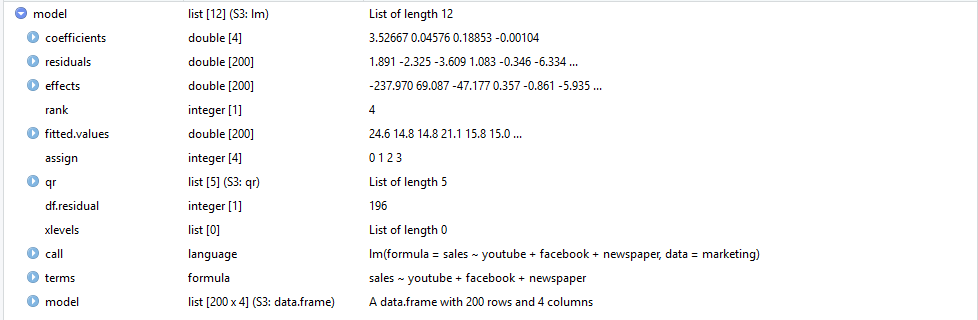
\includegraphics{lm.png}
\caption{}
\end{figure}

Strona w dokumentacji o funkcji \texttt{lm} -
\href{https://www.rdocumentation.org/packages/stats/versions/3.5.2/topics/lm}{link}.

\begin{figure}
\centering
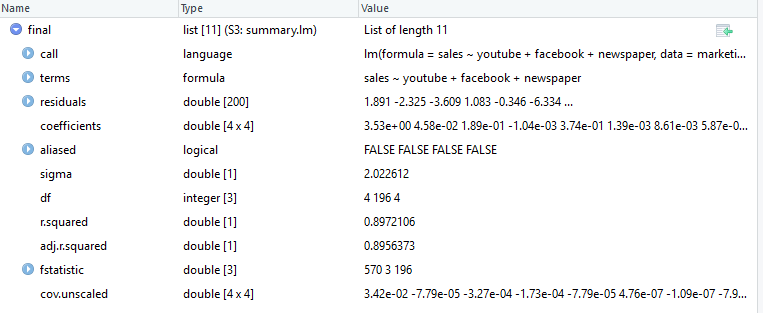
\includegraphics{summarylm.png}
\caption{}
\end{figure}

Sprawdźmy typ:

\begin{Shaded}
\begin{Highlighting}[]
\KeywordTok{class}\NormalTok{(model)}
\end{Highlighting}
\end{Shaded}

\begin{verbatim}
## [1] "lm"
\end{verbatim}

\begin{Shaded}
\begin{Highlighting}[]
\KeywordTok{class}\NormalTok{(final)}
\end{Highlighting}
\end{Shaded}

\begin{verbatim}
## [1] "summary.lm"
\end{verbatim}

\subsection{Współczynniki w modelu}\label{wspoczynniki-w-modelu}

Zapiszmy nasz model w postaci:

\[ y = X\beta + \varepsilon,\] gdzie: \[y = \begin{bmatrix}
y_1 \\ y_2 \\ \vdots \\ y_n
\end{bmatrix}, \quad  {X}=\begin{bmatrix}
X_{10} & X_{11} & X_{12} & \cdots & X_{1p} \\
X_{20} & X_{21} & X_{22} & \cdots & X_{2p} \\
\vdots & \vdots & \vdots & \ddots & \vdots \\
X_{n0} &X_{n1} & X_{n2} & \cdots & X_{np}
\end{bmatrix} ,
\quad  \beta = \begin{bmatrix}
\beta_0 \\ \beta_1 \\ \vdots \\ \beta_p \end{bmatrix}, \quad \varepsilon = \begin{bmatrix}
\varepsilon_1 \\ \varepsilon_2 \\ \vdots \\ \varepsilon_n
\end{bmatrix}\]

Na mocy konwencji \(x_{i0} = 1\) dla wszystkich \(i = 1, \ldots, n\).
Wtedy \(\beta_0\) jest wyrazem wolnym. Możemy też zapisać następująco:
\[y_i = \beta_0 +X_{i1}\beta_1+X_{i2}\beta_2+\ldots+X_{ip}\beta_p+\varepsilon_i, \quad i=1,\ldots, n.\]

Zazwyczaj taki układ równań nie ma rozwiązania. Naszym zadaniem jest
znalezienie możliwych wektorów \(\beta\), które ``dają najlepsze
dopasowanie''. Innymi słowy, musimy ``matematycznie'' rozwiązać problem
znalezienia
\[\hat{\beta}=\underset{\beta}{\operatorname{arg\,min}}\,S(\beta), \]
\[S(\beta) = \sum_{i=1}^n \bigl| y_i - \sum_{j=0}^p X_{ij}\beta_j\bigr|^2 = \bigl\| y -  X  \beta \bigr\|^2.\]
Rozwiązaniem jest: \[\hat{\beta}= ( X^T X )^{-1}  X^T  y.\]

Dowód: \href{https://en.wikipedia.org/wiki/Ordinary_least_squares}{wiki}
lub dowolny ``dobry'' podręcznik do zaawansowanej analizy matematycznej
lub/i statystyki.

Jak to policzyć dla ramki \texttt{marketing}?

\begin{Shaded}
\begin{Highlighting}[]
\NormalTok{x<-}\KeywordTok{cbind}\NormalTok{(}\KeywordTok{rep}\NormalTok{(}\DecValTok{1}\NormalTok{,}\DecValTok{200}\NormalTok{),}\KeywordTok{as.matrix}\NormalTok{(marketing[,}\KeywordTok{c}\NormalTok{(}\DecValTok{1}\NormalTok{,}\DecValTok{2}\NormalTok{,}\DecValTok{3}\NormalTok{)]))}
\NormalTok{y<-}\KeywordTok{as.matrix}\NormalTok{(marketing[,}\KeywordTok{c}\NormalTok{(}\DecValTok{4}\NormalTok{)])}
\NormalTok{betah =}\StringTok{ }\KeywordTok{solve}\NormalTok{(}\KeywordTok{t}\NormalTok{(x) }\OperatorTok\StringTok{ }\NormalTok{x) }\OperatorTok\StringTok{ }\NormalTok{(}\KeywordTok{t}\NormalTok{(x) }\OperatorTok\StringTok{ }\NormalTok{y)}
\NormalTok{betah}
\end{Highlighting}
\end{Shaded}

\begin{verbatim}
##                   [,1]
##            3.526667243
## youtube    0.045764645
## facebook   0.188530017
## newspaper -0.001037493
\end{verbatim}

\begin{Shaded}
\begin{Highlighting}[]
\NormalTok{model}\OperatorTok{$}\NormalTok{coefficients}
\end{Highlighting}
\end{Shaded}

\begin{verbatim}
##  (Intercept)      youtube     facebook    newspaper 
##  3.526667243  0.045764645  0.188530017 -0.001037493
\end{verbatim}

\begin{Shaded}
\begin{Highlighting}[]
\KeywordTok{summary}\NormalTok{(model)}\OperatorTok{$}\NormalTok{coefficients[,}\DecValTok{1}\NormalTok{]}
\end{Highlighting}
\end{Shaded}

\begin{verbatim}
##  (Intercept)      youtube     facebook    newspaper 
##  3.526667243  0.045764645  0.188530017 -0.001037493
\end{verbatim}

\begin{Shaded}
\begin{Highlighting}[]
\KeywordTok{coef}\NormalTok{(model)}
\end{Highlighting}
\end{Shaded}

\begin{verbatim}
##  (Intercept)      youtube     facebook    newspaper 
##  3.526667243  0.045764645  0.188530017 -0.001037493
\end{verbatim}

\begin{Shaded}
\begin{Highlighting}[]
\NormalTok{betah}\OperatorTok{-}\NormalTok{model}\OperatorTok{$}\NormalTok{coefficients}
\end{Highlighting}
\end{Shaded}

\begin{verbatim}
##                    [,1]
##           -6.838974e-14
## youtube    2.428613e-16
## facebook  -3.885781e-16
## newspaper  5.861197e-16
\end{verbatim}

\subsection{Błąd standardowy regresji}\label{bad-standardowy-regresji}

Dopasowane wartości (przewidywane wartości) - wartości otrzymane poprzez
model: \[\hat{y}=X\hat{\beta}=Py, \quad P=X(X^TX)^{-1}X^T.\] Zróbmy to w
R:

\begin{Shaded}
\begin{Highlighting}[]
\NormalTok{yh<-x }\OperatorTok\StringTok{ }\NormalTok{betah}
\NormalTok{p<-x }\OperatorTok\StringTok{  }\KeywordTok{solve}\NormalTok{(}\KeywordTok{t}\NormalTok{(x) }\OperatorTok\StringTok{ }\NormalTok{x) }\OperatorTok\StringTok{ }\KeywordTok{t}\NormalTok{(x)}
\NormalTok{yh2<-}\StringTok{ }\NormalTok{p }\OperatorTok\StringTok{ }\NormalTok{y}
\NormalTok{yh3<-model}\OperatorTok{$}\NormalTok{fitted.values}
\KeywordTok{head}\NormalTok{(}\KeywordTok{cbind}\NormalTok{(yh,yh2,yh3))}
\end{Highlighting}
\end{Shaded}

\begin{verbatim}
##                          yh3
## 1 24.62877 24.62877 24.62877
## 2 14.80543 14.80543 14.80543
## 3 14.76920 14.76920 14.76920
## 4 21.11740 21.11740 21.11740
## 5 15.82641 15.82641 15.82641
## 6 14.97402 14.97402 14.97402
\end{verbatim}

Zauważmy, że \(PX=X\) oraz \(PX-X=0\). Niech \(M=I_n-P\). Wtedy
\(MX=0\). Macierz \(M\) nazywamy macierzą anihilującą.

W R mamy:

\begin{Shaded}
\begin{Highlighting}[]
\KeywordTok{head}\NormalTok{(p }\OperatorTok\StringTok{ }\NormalTok{x)}
\end{Highlighting}
\end{Shaded}

\begin{verbatim}
##        youtube facebook newspaper
## [1,] 1  276.12    45.36     83.04
## [2,] 1   53.40    47.16     54.12
## [3,] 1   20.64    55.08     83.16
## [4,] 1  181.80    49.56     70.20
## [5,] 1  216.96    12.96     70.08
## [6,] 1   10.44    58.68     90.00
\end{verbatim}

\begin{Shaded}
\begin{Highlighting}[]
\KeywordTok{head}\NormalTok{(x)}
\end{Highlighting}
\end{Shaded}

\begin{verbatim}
##        youtube facebook newspaper
## [1,] 1  276.12    45.36     83.04
## [2,] 1   53.40    47.16     54.12
## [3,] 1   20.64    55.08     83.16
## [4,] 1  181.80    49.56     70.20
## [5,] 1  216.96    12.96     70.08
## [6,] 1   10.44    58.68     90.00
\end{verbatim}

\begin{Shaded}
\begin{Highlighting}[]
\NormalTok{m<-}\KeywordTok{diag}\NormalTok{(}\DecValTok{200}\NormalTok{)}\OperatorTok{-}\NormalTok{p}
\KeywordTok{head}\NormalTok{(m }\OperatorTok\StringTok{ }\NormalTok{x)}
\end{Highlighting}
\end{Shaded}

\begin{verbatim}
##                          youtube      facebook    newspaper
## [1,] -1.882175e-16 -1.170453e-13 -2.310565e-14 5.541834e-14
## [2,]  2.740863e-16  4.223288e-13 -4.801715e-15 4.510281e-15
## [3,] -1.526557e-15  2.353673e-13 -4.754530e-14 1.862399e-14
## [4,] -2.359224e-16  2.091660e-13 -1.249001e-15 4.567874e-14
## [5,]  1.023487e-16 -3.175238e-14 -2.490369e-14 7.316370e-14
## [6,] -1.242062e-15  3.108624e-13 -3.716472e-14 5.159762e-14
\end{verbatim}

Teraz możemy obliczć reszty (residua):

\[ \hat{\varepsilon} = y - \hat{y} = y - X\hat{\beta} = My = M(X\beta+\varepsilon) = (MX)\beta + M\varepsilon = M\varepsilon.\]
W R wygląda to następująco:

\begin{Shaded}
\begin{Highlighting}[]
\NormalTok{eh<-y}\OperatorTok{-}\NormalTok{yh}
\KeywordTok{head}\NormalTok{(eh)}
\end{Highlighting}
\end{Shaded}

\begin{verbatim}
##            [,1]
## [1,]  1.8912307
## [2,] -2.3254258
## [3,] -3.6092049
## [4,]  1.0826046
## [5,] -0.3464062
## [6,] -6.3340172
\end{verbatim}

\begin{Shaded}
\begin{Highlighting}[]
\KeywordTok{quantile}\NormalTok{(eh)}
\end{Highlighting}
\end{Shaded}

\begin{verbatim}
##          0%         25%         50%         75%        100% 
## -10.5932245  -1.0689763   0.2901621   1.4271824   3.3950671
\end{verbatim}

\begin{Shaded}
\begin{Highlighting}[]
\KeywordTok{quantile}\NormalTok{(model}\OperatorTok{$}\NormalTok{residuals)}
\end{Highlighting}
\end{Shaded}

\begin{verbatim}
##          0%         25%         50%         75%        100% 
## -10.5932245  -1.0689763   0.2901621   1.4271824   3.3950671
\end{verbatim}

\begin{Shaded}
\begin{Highlighting}[]
\KeywordTok{quantile}\NormalTok{(}\KeywordTok{summary}\NormalTok{(model)}\OperatorTok{$}\NormalTok{residuals)}
\end{Highlighting}
\end{Shaded}

\begin{verbatim}
##          0%         25%         50%         75%        100% 
## -10.5932245  -1.0689763   0.2901621   1.4271824   3.3950671
\end{verbatim}

Dzięki resztom możemy estymować wariancję:

\[s^2 = \frac{\hat{\varepsilon} ^T \hat{\varepsilon}}{n-p} = \frac{(My)^T My}{n-p} = \frac{y^T M^TMy}{n-p}= \frac{y ^T My}{n-p} = \frac{S(\hat{\beta})}{n-p},\quad
    \hat\sigma^2 = \frac{n-p}{n}\;s^2\] U nas \(n=200\) i \(p=4\)
(liczba zmiennych plus 1 zgodnie z konwencją). Liczba \(n-p\) odpowiada
``w ujęciu statystycznym'' liczbie stopni swobody.

W R mamy:

\begin{Shaded}
\begin{Highlighting}[]
\NormalTok{s2<-}\StringTok{ }\KeywordTok{t}\NormalTok{(eh) }\OperatorTok\StringTok{ }\NormalTok{eh }\OperatorTok{/}\DecValTok{196}
\NormalTok{s2<-}\KeywordTok{as.numeric}\NormalTok{(s2)}
\KeywordTok{sqrt}\NormalTok{(s2)}
\end{Highlighting}
\end{Shaded}

\begin{verbatim}
## [1] 2.022612
\end{verbatim}

\begin{Shaded}
\begin{Highlighting}[]
\NormalTok{sigmah2<-}\DecValTok{196}\OperatorTok{/}\DecValTok{200}\OperatorTok{*}\NormalTok{s2}
\KeywordTok{sqrt}\NormalTok{(sigmah2)}
\end{Highlighting}
\end{Shaded}

\begin{verbatim}
## [1] 2.002284
\end{verbatim}

\emph{\(s^2\) jest nieobciążonym estymatorem wariancji przy użyciu
metody najmniejszych kwadratów. \(\hat{\sigma}^2\) jest obciążonym
estymatorem wariancji przy użyciu metody najmniejszej wiarygodności.
Częściej jest używane \(s^2\).}

\begin{Shaded}
\begin{Highlighting}[]
\KeywordTok{summary}\NormalTok{(model)}\OperatorTok{$}\NormalTok{sigma}
\end{Highlighting}
\end{Shaded}

\begin{verbatim}
## [1] 2.022612
\end{verbatim}

\(s^2\) nazywa się odchyleniem standardowym składnika resztowego, błędem
standardowym regresji, odchyleniem standardowym regresji\ldots{}

\subsection{\texorpdfstring{``Dobroć''
dopasowania}{Dobroć dopasowania}}\label{dobroc-dopasowania}

Współczynnik determinacji:

\[ R^2 = \frac{\sum(\hat{y}_i-\overline{y})^2}{\sum(y_i-\overline{y})^2} = \frac{y ^T P ^T LPy}{y ^T Ly} = 1 - \frac{y^T My}{y^T Ly} = 1 - \frac{ SSR}{SST} = \frac{SSM}{SST},\]
gdzie \(L=I_n - \mathbf{1}\mathbf{1}^T/n\), a \(\mathbf{1}\) to macierz
wymiaru \(n\times 1\) składająca się z samych jedynek. \(SST\) -
całkowita (totalna) suma kwadratów, \(SSR\) - suma kwadratów reszt
(błędów), \(SSM\) - skorygowana suma kwadratów dla modelu.

W R mamy:

\begin{Shaded}
\begin{Highlighting}[]
\NormalTok{ym=}\KeywordTok{mean}\NormalTok{(y)}
\NormalTok{ssm<-}\KeywordTok{sum}\NormalTok{((yh}\OperatorTok{-}\NormalTok{ym)}\OperatorTok{^}\DecValTok{2}\NormalTok{)}
\NormalTok{sst<-}\KeywordTok{sum}\NormalTok{((y}\OperatorTok{-}\NormalTok{ym)}\OperatorTok{^}\DecValTok{2}\NormalTok{)}
\NormalTok{r2<-ssm}\OperatorTok{/}\NormalTok{sst}
\NormalTok{r2}
\end{Highlighting}
\end{Shaded}

\begin{verbatim}
## [1] 0.8972106
\end{verbatim}

\begin{Shaded}
\begin{Highlighting}[]
\NormalTok{one<-}\KeywordTok{matrix}\NormalTok{( }\KeywordTok{rep}\NormalTok{( }\DecValTok{1}\NormalTok{, }\DataTypeTok{len=}\DecValTok{200}\NormalTok{), }\DataTypeTok{nrow =} \DecValTok{200}\NormalTok{)}
\NormalTok{l<-}\KeywordTok{diag}\NormalTok{(}\DecValTok{200}\NormalTok{)}\OperatorTok{-}\StringTok{ }\NormalTok{one }\OperatorTok\StringTok{ }\KeywordTok{t}\NormalTok{(one) }\OperatorTok{/}\DecValTok{200}
\KeywordTok{t}\NormalTok{(y) }\OperatorTok\StringTok{ }\KeywordTok{t}\NormalTok{(p) }\OperatorTok\StringTok{ }\NormalTok{l }\OperatorTok\StringTok{ }\NormalTok{p }\OperatorTok\StringTok{ }\NormalTok{y }\OperatorTok{/}\StringTok{ }\NormalTok{(}\KeywordTok{t}\NormalTok{(y) }\OperatorTok\StringTok{ }\NormalTok{l }\OperatorTok\StringTok{ }\NormalTok{y)}
\end{Highlighting}
\end{Shaded}

\begin{verbatim}
##           [,1]
## [1,] 0.8972106
\end{verbatim}

\begin{Shaded}
\begin{Highlighting}[]
\DecValTok{1}\OperatorTok{-}\StringTok{ }\KeywordTok{t}\NormalTok{(y) }\OperatorTok\StringTok{ }\NormalTok{m }\OperatorTok\StringTok{ }\NormalTok{y }\OperatorTok{/}\NormalTok{(}\KeywordTok{t}\NormalTok{(y) }\OperatorTok\StringTok{ }\NormalTok{l }\OperatorTok\StringTok{ }\NormalTok{y)}
\end{Highlighting}
\end{Shaded}

\begin{verbatim}
##           [,1]
## [1,] 0.8972106
\end{verbatim}

\begin{Shaded}
\begin{Highlighting}[]
\KeywordTok{summary}\NormalTok{(model)}\OperatorTok{$}\NormalTok{r.squared}
\end{Highlighting}
\end{Shaded}

\begin{verbatim}
## [1] 0.8972106
\end{verbatim}

Skorygowany współczynnik determinacji:

\[\overline{R}^2=1 - (1 - R^2) \frac{n - 1}{n - p}\] W R mamy:

\begin{Shaded}
\begin{Highlighting}[]
\NormalTok{ro2<-}\DecValTok{1}\OperatorTok{-}\NormalTok{((}\DecValTok{1}\OperatorTok{-}\NormalTok{r2)}\OperatorTok{*}\NormalTok{(}\DecValTok{199}\OperatorTok{/}\DecValTok{196}\NormalTok{))}
\NormalTok{ro2}
\end{Highlighting}
\end{Shaded}

\begin{verbatim}
## [1] 0.8956373
\end{verbatim}

\begin{Shaded}
\begin{Highlighting}[]
\KeywordTok{summary}\NormalTok{(model)}\OperatorTok{$}\NormalTok{adj.r.squared}
\end{Highlighting}
\end{Shaded}

\begin{verbatim}
## [1] 0.8956373
\end{verbatim}

\subsection{F-test}\label{f-test}

Powtórzmy i wprowadźmy nowe oznaczenia:

\begin{itemize}
\tightlist
\item
  \(n\) - liczba obserwacji
\item
  \(p\) - liczba parametrów regresji (w modelu liniowym to liczba
  zmiennych objaśniająch+1 zgodnie z konwencją)
\item
  \(SSM\) - skorygowana suma kwadratów modelu
  \[SSM=\sum_{i=1}^n ( \hat{y}_i-\overline{y} )^2\]
\end{itemize}

\begin{Shaded}
\begin{Highlighting}[]
\NormalTok{ssm<-}\KeywordTok{sum}\NormalTok{((yh}\OperatorTok{-}\NormalTok{ym)}\OperatorTok{^}\DecValTok{2}\NormalTok{)}
\NormalTok{ssm}
\end{Highlighting}
\end{Shaded}

\begin{verbatim}
## [1] 6998.866
\end{verbatim}

\begin{itemize}
\tightlist
\item
  \(SSR \ (SSE)\) - suma kwadratów reszt, błędów
\end{itemize}

\[SSR=\sum_{i=1}^n ( y_i-\hat{y}_i )^2\]

\begin{Shaded}
\begin{Highlighting}[]
\NormalTok{ssr<-}\KeywordTok{sum}\NormalTok{((y}\OperatorTok{-}\NormalTok{yh)}\OperatorTok{^}\DecValTok{2}\NormalTok{)}
\NormalTok{ssr}
\end{Highlighting}
\end{Shaded}

\begin{verbatim}
## [1] 801.8284
\end{verbatim}

\begin{itemize}
\tightlist
\item
  \(SST\) - skorygowana totalna (całkowita) suma kwadratów
\end{itemize}

\[ SST = \sum_{i=1}^n ( y_i-\overline{y} )^2\]

\begin{Shaded}
\begin{Highlighting}[]
\NormalTok{sst<-}\KeywordTok{sum}\NormalTok{((y}\OperatorTok{-}\NormalTok{ym)}\OperatorTok{^}\DecValTok{2}\NormalTok{)}
\NormalTok{sst}
\end{Highlighting}
\end{Shaded}

\begin{verbatim}
## [1] 7800.694
\end{verbatim}

Zachodzi równość: \[SSM+SSR=SST\]

\begin{Shaded}
\begin{Highlighting}[]
\NormalTok{ssm}\OperatorTok{+}\NormalTok{ssr}
\end{Highlighting}
\end{Shaded}

\begin{verbatim}
## [1] 7800.694
\end{verbatim}

\begin{itemize}
\tightlist
\item
  \(DFM\) - skorygowane stopnie swobody modelu (u nas w modelu liniowym
  liczba zmiennych objaśniających), \(DFM=p-1\)
\item
  \(DFE\) - stopnie swobody błędu, \(DFE=n-p\)
\item
  \(DFT\) - skorygowane totalne (całkowite) stopnie swobody, \(DFT=n-1\)
\end{itemize}

Zachodzi: \[DFM + DFE = DFT.\] * \(MSM\) - średnia kwadratów modelu,
\(MSM = SSM / DFM\)

\begin{Shaded}
\begin{Highlighting}[]
\NormalTok{msm<-ssm}\OperatorTok{/}\DecValTok{3}
\NormalTok{msm}
\end{Highlighting}
\end{Shaded}

\begin{verbatim}
## [1] 2332.955
\end{verbatim}

\begin{itemize}
\tightlist
\item
  \(MSE\) - średnia kwadratów błędów, \(MSE = SSR / DFE\)
\end{itemize}

\begin{Shaded}
\begin{Highlighting}[]
\NormalTok{mse<-ssr}\OperatorTok{/}\DecValTok{196}
\NormalTok{mse}
\end{Highlighting}
\end{Shaded}

\begin{verbatim}
## [1] 4.090961
\end{verbatim}

\begin{itemize}
\tightlist
\item
  \(MST\) - totalna (całkowita) średnia kwadratów, \(MST = SST / DFT\)
\end{itemize}

\begin{Shaded}
\begin{Highlighting}[]
\NormalTok{mst<-sst}\OperatorTok{/}\DecValTok{199}
\NormalTok{mst}
\end{Highlighting}
\end{Shaded}

\begin{verbatim}
## [1] 39.19947
\end{verbatim}

\textbf{F-test dla regresji wielowymiarowej}

\[H_0: \qquad   \beta_1 = \beta_2 = \ldots = \beta_{p-1} = 0\]

\[H_1: \qquad  \beta_j \neq 0 \ \mathrm{dla \ co \ najmniej \ jednego} \ j.\]
Wyliczamy statystykę:

\[F=\frac{MSM}{MSE} = \frac{\mathrm{"wyjaśniona \ wariancja"}}{\mathrm{"niewyjaśniona \ wariancja"}} \]

\begin{Shaded}
\begin{Highlighting}[]
\NormalTok{f<-msm}\OperatorTok{/}\NormalTok{mse}
\NormalTok{f}
\end{Highlighting}
\end{Shaded}

\begin{verbatim}
## [1] 570.2707
\end{verbatim}

\begin{Shaded}
\begin{Highlighting}[]
\KeywordTok{summary}\NormalTok{(model)}\OperatorTok{$}\NormalTok{fstatistic}
\end{Highlighting}
\end{Shaded}

\begin{verbatim}
##    value    numdf    dendf 
## 570.2707   3.0000 196.0000
\end{verbatim}

Statystyka ta podlega rozkładowi F-Snedecora z \(p-1\) i \(n-p\)
stopniami swobody. Ustalamy \(\alpha=0,05\).

\begin{Shaded}
\begin{Highlighting}[]
\KeywordTok{qf}\NormalTok{(}\FloatTok{0.95}\NormalTok{, }\DecValTok{3}\NormalTok{, }\DecValTok{196}\NormalTok{)}
\end{Highlighting}
\end{Shaded}

\begin{verbatim}
## [1] 2.650677
\end{verbatim}

Jeśli wartość statystyki jest większa kwantylowi, odrzucamy hipotezę
zerową. W przeciwnym wypadku przyjmujemy hipotezę zerową.

W naszym wypadku odrzucamy hipotezę zerową. Innymi słowy, odrzucamy
hipotezę że wydatki na reklamy na poszczególne media nie mają wpływu na
sprzedaż.

Obliczmy wartość \(p\):

\begin{Shaded}
\begin{Highlighting}[]
\NormalTok{p<-}\DecValTok{1}\OperatorTok{-}\KeywordTok{pf}\NormalTok{(f, }\DecValTok{3}\NormalTok{,}\DecValTok{196}\NormalTok{)}
\NormalTok{p}
\end{Highlighting}
\end{Shaded}

\begin{verbatim}
## [1] 0
\end{verbatim}

\begin{Shaded}
\begin{Highlighting}[]
\NormalTok{fstat<-}\KeywordTok{summary}\NormalTok{(model)}\OperatorTok{$}\NormalTok{fstatistic }
\DecValTok{1}\OperatorTok{-}\KeywordTok{pf}\NormalTok{(fstat[}\DecValTok{1}\NormalTok{], fstat[}\DecValTok{2}\NormalTok{],fstat[}\DecValTok{3}\NormalTok{])}
\end{Highlighting}
\end{Shaded}

\begin{verbatim}
## value 
##     0
\end{verbatim}

W naszym wypadku jest to ``bliskie'' zeru``, więc możemy przyjąć, że się
zgadza.

Jeśli \(p\leqslant \alpha\) odrzucamy \(H_0\) przyjując \(H_1\). W
przeciwnym wypadku nie ma podstaw by odrzucić \(H_0\).

\subsection{t-test}\label{t-test}

Przypomnijmy, że \[\hat{\beta}= ( X^T X )^{-1}  X^T  y.\]

Wariancja wektora współczynników:
\[\operatorname(VAR) (\hat{\beta}) = \sigma^2 (X^TX)^{-1}.\] Zamieniając
na esytmator nieobciążony:
\[\widehat{\operatorname(VAR)}(\hat{\beta}) = s^2 (X^TX)^{-1} \] By
otrzymać odchylenie standardowe poszczególnych współczynników, wybieramy
elementy na głównej przekątnej ostatniej macierzy i potem je
pierwiastkujemy.

\begin{Shaded}
\begin{Highlighting}[]
\NormalTok{v<-s2 }\OperatorTok{*}\StringTok{ }\KeywordTok{solve}\NormalTok{(}\KeywordTok{t}\NormalTok{(x) }\OperatorTok\StringTok{ }\NormalTok{x)}
\NormalTok{v}
\end{Highlighting}
\end{Shaded}

\begin{verbatim}
##                               youtube      facebook     newspaper
##            0.1400929170 -3.188728e-04 -1.338587e-03 -7.092255e-04
## youtube   -0.0003188728  1.945737e-06 -4.470395e-07 -3.265950e-07
## facebook  -0.0013385874 -4.470395e-07  7.415335e-05 -1.780062e-05
## newspaper -0.0007092255 -3.265950e-07 -1.780062e-05  3.446875e-05
\end{verbatim}

\begin{Shaded}
\begin{Highlighting}[]
\KeywordTok{vcov}\NormalTok{(model)}
\end{Highlighting}
\end{Shaded}

\begin{verbatim}
##               (Intercept)       youtube      facebook     newspaper
## (Intercept)  0.1400929170 -3.188728e-04 -1.338587e-03 -7.092255e-04
## youtube     -0.0003188728  1.945737e-06 -4.470395e-07 -3.265950e-07
## facebook    -0.0013385874 -4.470395e-07  7.415335e-05 -1.780062e-05
## newspaper   -0.0007092255 -3.265950e-07 -1.780062e-05  3.446875e-05
\end{verbatim}

\begin{Shaded}
\begin{Highlighting}[]
\NormalTok{varbeta<-}\KeywordTok{sqrt}\NormalTok{(}\KeywordTok{diag}\NormalTok{(v))}
\KeywordTok{sqrt}\NormalTok{(}\KeywordTok{diag}\NormalTok{(}\KeywordTok{vcov}\NormalTok{(model)))}
\end{Highlighting}
\end{Shaded}

\begin{verbatim}
## (Intercept)     youtube    facebook   newspaper 
## 0.374289884 0.001394897 0.008611234 0.005871010
\end{verbatim}

\begin{Shaded}
\begin{Highlighting}[]
\KeywordTok{summary}\NormalTok{(model)}\OperatorTok{$}\NormalTok{coefficients[,}\DecValTok{2}\NormalTok{]}
\end{Highlighting}
\end{Shaded}

\begin{verbatim}
## (Intercept)     youtube    facebook   newspaper 
## 0.374289884 0.001394897 0.008611234 0.005871010
\end{verbatim}

Statystykę \(t\) określamy następująco:
\[t=\frac{\hat{\beta}}{\widehat{\operatorname(VAR)}(\hat{\beta})}\]

\begin{Shaded}
\begin{Highlighting}[]
\NormalTok{tstat<-betah}\OperatorTok{/}\NormalTok{varbeta}
\NormalTok{tstat}
\end{Highlighting}
\end{Shaded}

\begin{verbatim}
##                 [,1]
##            9.4222884
## youtube   32.8086244
## facebook  21.8934961
## newspaper -0.1767146
\end{verbatim}

\begin{Shaded}
\begin{Highlighting}[]
\KeywordTok{summary}\NormalTok{(model)}\OperatorTok{$}\NormalTok{coefficients[,}\DecValTok{3}\NormalTok{]}
\end{Highlighting}
\end{Shaded}

\begin{verbatim}
## (Intercept)     youtube    facebook   newspaper 
##   9.4222884  32.8086244  21.8934961  -0.1767146
\end{verbatim}

Na koniec liczymy odpowiednie prawopodobieństwo (liczba stopni swobody
to \(n-p\):

\begin{Shaded}
\begin{Highlighting}[]
\DecValTok{2} \OperatorTok{*}\StringTok{ }\KeywordTok{pt}\NormalTok{(}\KeywordTok{abs}\NormalTok{(tstat), }\DecValTok{196}\NormalTok{, }\DataTypeTok{lower.tail =} \OtherTok{FALSE}\NormalTok{)}
\end{Highlighting}
\end{Shaded}

\begin{verbatim}
##                   [,1]
##           1.267295e-17
## youtube   1.509960e-81
## facebook  1.505339e-54
## newspaper 8.599151e-01
\end{verbatim}

\begin{Shaded}
\begin{Highlighting}[]
\KeywordTok{summary}\NormalTok{(model)}\OperatorTok{$}\NormalTok{coefficients[,}\DecValTok{4}\NormalTok{]}
\end{Highlighting}
\end{Shaded}

\begin{verbatim}
##  (Intercept)      youtube     facebook    newspaper 
## 1.267295e-17 1.509960e-81 1.505339e-54 8.599151e-01
\end{verbatim}

Test \(t\) pozwala zweryfikować istotność oszacownia parametru dla
każdej ze zmiennej objaśniającej. \[H_0: \qquad \beta_i=0\]
\[H_1: \qquad \beta_i\neq 0\]

Jeśli prawodpobieństwo jest większe niż poziom ufności (domyślnie
\(\alpha=0,05\)) to odrzucamy \(H_0\) na rzecz \(H_1\). W przeciwnym
wypadku nie mamy podstaw do odrzucenia \(H_0\).

W rozważanym przykładzie jedynie w przypadku zmiennej \texttt{newspaper}
odrzucamy \(H_0\). Nie jest zatem znacząca w modelu regresji
wielokrotnej. Oznacza to, że w przypadku ustalonej kwoty budżetu
reklamowego \texttt{youtube} i \texttt{facebook} zmiany w budżecie
reklamowym newspaper nie wpłyną znacząco na wyniki sprzedaży. Możemy
zatem zmienną \texttt{newspaper} usunąć z modelu:

\begin{Shaded}
\begin{Highlighting}[]
\NormalTok{model2  <-}\StringTok{ }\KeywordTok{lm}\NormalTok{(sales }\OperatorTok{~}\StringTok{ }\NormalTok{youtube }\OperatorTok{+}\StringTok{ }\NormalTok{facebook, }\DataTypeTok{data =}\NormalTok{ marketing)}
\KeywordTok{summary}\NormalTok{(model2)}
\end{Highlighting}
\end{Shaded}

\begin{verbatim}
## 
## Call:
## lm(formula = sales ~ youtube + facebook, data = marketing)
## 
## Residuals:
##      Min       1Q   Median       3Q      Max 
## -10.5572  -1.0502   0.2906   1.4049   3.3994 
## 
## Coefficients:
##             Estimate Std. Error t value Pr(>|t|)    
## (Intercept)  3.50532    0.35339   9.919   <2e-16 ***
## youtube      0.04575    0.00139  32.909   <2e-16 ***
## facebook     0.18799    0.00804  23.382   <2e-16 ***
## ---
## Signif. codes:  0 '***' 0.001 '**' 0.01 '*' 0.05 '.' 0.1 ' ' 1
## 
## Residual standard error: 2.018 on 197 degrees of freedom
## Multiple R-squared:  0.8972, Adjusted R-squared:  0.8962 
## F-statistic: 859.6 on 2 and 197 DF,  p-value: < 2.2e-16
\end{verbatim}

\section{Inne zapisy}\label{inne-zapisy}

W R możemy wywołać modele nieco inną składnią:

\begin{Shaded}
\begin{Highlighting}[]
\NormalTok{model3 <-}\StringTok{ }\KeywordTok{lm}\NormalTok{(sales }\OperatorTok{~}\NormalTok{., }\DataTypeTok{data =}\NormalTok{ marketing)}
\KeywordTok{summary}\NormalTok{(model3)}
\end{Highlighting}
\end{Shaded}

\begin{verbatim}
## 
## Call:
## lm(formula = sales ~ ., data = marketing)
## 
## Residuals:
##      Min       1Q   Median       3Q      Max 
## -10.5932  -1.0690   0.2902   1.4272   3.3951 
## 
## Coefficients:
##              Estimate Std. Error t value Pr(>|t|)    
## (Intercept)  3.526667   0.374290   9.422   <2e-16 ***
## youtube      0.045765   0.001395  32.809   <2e-16 ***
## facebook     0.188530   0.008611  21.893   <2e-16 ***
## newspaper   -0.001037   0.005871  -0.177     0.86    
## ---
## Signif. codes:  0 '***' 0.001 '**' 0.01 '*' 0.05 '.' 0.1 ' ' 1
## 
## Residual standard error: 2.023 on 196 degrees of freedom
## Multiple R-squared:  0.8972, Adjusted R-squared:  0.8956 
## F-statistic: 570.3 on 3 and 196 DF,  p-value: < 2.2e-16
\end{verbatim}

\begin{Shaded}
\begin{Highlighting}[]
\NormalTok{model4 <-}\StringTok{ }\KeywordTok{lm}\NormalTok{(sales }\OperatorTok{~}\NormalTok{. }\OperatorTok{-}\NormalTok{newspaper, }\DataTypeTok{data =}\NormalTok{ marketing)}
\KeywordTok{summary}\NormalTok{(model4)}
\end{Highlighting}
\end{Shaded}

\begin{verbatim}
## 
## Call:
## lm(formula = sales ~ . - newspaper, data = marketing)
## 
## Residuals:
##      Min       1Q   Median       3Q      Max 
## -10.5572  -1.0502   0.2906   1.4049   3.3994 
## 
## Coefficients:
##             Estimate Std. Error t value Pr(>|t|)    
## (Intercept)  3.50532    0.35339   9.919   <2e-16 ***
## youtube      0.04575    0.00139  32.909   <2e-16 ***
## facebook     0.18799    0.00804  23.382   <2e-16 ***
## ---
## Signif. codes:  0 '***' 0.001 '**' 0.01 '*' 0.05 '.' 0.1 ' ' 1
## 
## Residual standard error: 2.018 on 197 degrees of freedom
## Multiple R-squared:  0.8972, Adjusted R-squared:  0.8962 
## F-statistic: 859.6 on 2 and 197 DF,  p-value: < 2.2e-16
\end{verbatim}

\begin{Shaded}
\begin{Highlighting}[]
\NormalTok{model5 <-}\StringTok{ }\KeywordTok{lm}\NormalTok{(marketing}\OperatorTok{$}\NormalTok{sales}\OperatorTok{~}\StringTok{ }\NormalTok{marketing}\OperatorTok{$}\NormalTok{youtube }\OperatorTok{+}\StringTok{ }\NormalTok{marketing}\OperatorTok{$}\NormalTok{facebook)}
\KeywordTok{summary}\NormalTok{(model5)}
\end{Highlighting}
\end{Shaded}

\begin{verbatim}
## 
## Call:
## lm(formula = marketing$sales ~ marketing$youtube + marketing$facebook)
## 
## Residuals:
##      Min       1Q   Median       3Q      Max 
## -10.5572  -1.0502   0.2906   1.4049   3.3994 
## 
## Coefficients:
##                    Estimate Std. Error t value Pr(>|t|)    
## (Intercept)         3.50532    0.35339   9.919   <2e-16 ***
## marketing$youtube   0.04575    0.00139  32.909   <2e-16 ***
## marketing$facebook  0.18799    0.00804  23.382   <2e-16 ***
## ---
## Signif. codes:  0 '***' 0.001 '**' 0.01 '*' 0.05 '.' 0.1 ' ' 1
## 
## Residual standard error: 2.018 on 197 degrees of freedom
## Multiple R-squared:  0.8972, Adjusted R-squared:  0.8962 
## F-statistic: 859.6 on 2 and 197 DF,  p-value: < 2.2e-16
\end{verbatim}

\section{Założenia modelu}\label{zaozenia-modelu}

\begin{itemize}
\item
  \textbf{Istnienie}: Dla każdej kombinacji wartości zmiennych
  objaśniających \(X_1, X_2,\ldots, X_k\), zmienna objaśniana \(Y\) jest
  (jednoznaczną) zmienną losową z określonym rozkładem
  prawdopodobieństwa posiadającym skończoną wartość oczekiwaną i
  wariancję.
\item
  \textbf{Kontrolowanie wartości czynników}: Zmienną losową jest zmienna
  \(Y\), podczas gdy zmienne \(X_1, X_2,\ldots, X_k\) są zmiennymi
  (nielosowymi) kontrolowanymi.
\item
  \textbf{Liniowość}:
\item
  \textbf{Niezależność}: Obserwacje zmiennej objaśnianej \(Y\) są od
  siebie niezależne, tzn. poszczególne obserwacje zmiennej \(Y\) nie
  zależą od wartości otrzymanych wcześniej.
\item
  \textbf{Stałość rozproszenia (homoscedastyczność)}: Wariancja
  (warunkowa) zmiennej \(Y\) dla dowolnej ustalonej kombinacji zmiennych
  \(X_1, X_2,\ldots, X_k\) jest taka sama (jednorodna) dla wszystkich
  rozkładów warunkowych
\item
  \textbf{Normalność}: Dla dowolnej ustalonej liniowej kombinacji
  zmiennych \(X_1, X_2,\ldots, X_k\), zmienna \(Y\) ma rozkład normalny
\end{itemize}

\section{Na koniec}\label{na-koniec}

\begin{figure}
\centering
\includegraphics{https://sadlaff.files.wordpress.com/2014/02/sad-laff-working-from-home-joke1-e1392532216836.jpg}
\caption{}
\end{figure}


\end{document}
